\chapter{Docker Swarm}\label{ch:dockerswarm}

Nachdem ein Dockerfile für einen Microservice erstellt und das Image gebaut wurde, ist der nächste Schritt das Ausliefern der Software. 
Während Docker Container lokal zum Testen problemlos einzeln über die Kommandozeile oder auch als Gesamtpaket per Docker Compose-Datei gestartet werden können, ist dies für Test- und Produktivumgebungen mühselig und unpraktikabel zu pflegen. 
Die Container einmalig zu starten, ist schließlich nur der Anfang.
H\"aufig besteht eine Software aus mehreren Microservices, die \"uber mehrere Hosts verteilt sind. 
Über die Lebensdauer einer Software hinweg, muss kontrolliert werden, ob der Container fehlerfrei läuft und dass er nicht abstürzt, um die Verfügbarkeit zu gewährleisten.
Unter Umständen müssen mehrere Container-Instanzen gestartet werden, um einer höheren Last standhalten zu können. 
Zudem muss die Kommunikation zwischen einzelnen Containern und zwischen Containern und der Außenwelt sichergestellt werden. 

All diese Punkte ergeben zusammen die sogenannte Containerorchestrierung. 
Diese Tätigkeit kann manuell ausgeführt werden, aber im Zeitalter der Automatisierung und DevOps-Kultur gibt es dafür selbstverständlich bessere Optionen. 
Am weitesten verbreitet ist hierbei das System Kubernetes, das von Google entwickelt wurde, aber schon von Anfang an der Community als Open-Source-Projekt zur Verfügung gestellt wurde. 
Es dient der automatisierten Bereitstellung, Skalierung und Verwaltung von containerisierten Anwendungen, bietet aber darüber hinaus viele weitere Optionen.

Entsprechend ist die Software recht komplex und kann anfangs inbesondere f\"ur Einsteigerinnen eine Herausforderung darstellen. 
Alternativ dazu gibt es eine hauseigene Plattform zur Containerorchestrierung von Docker selber, den Docker Swarm Mode. 
Ein Swarm ist ein Cluster bestehend aus einer oder mehrerer Docker Engines verteilt auf mehreren Servern oder virtuellen Maschinen.\cite{Docker_Engine_Swarm}
Der Docker Swarm Mode ist seit 2016 nativ ein Teil von Docker, aber standardm\"a{\ss}ig ausgeschaltet.
Der folgende Abschnitt beleuchtet den Aufbau und die Funktionsweise dieser Plattform.  

\section{Nodes}

Die einzelnen Docker Engines, die Teil eines Swarms sind, werden als Nodes bezeichnet. 
Jede Node hat zur Laufzeit entweder die Rolle eines Managers oder Workers, wobei die Rollen dynamisch durch User ge\"andert werden k\"onnen. 

Ein Manager-Node ist daf\"ur zust\"andig, mithilfe des Raft-Algorithmus den internen Zustand des Swarms zu erhalten, also bswp.\ die Anzahl an definierten Containern eines bestimmten Services sicherzustellen und einen neuen Container hochzufahren, wenn einer fehlschl\"agt. 
Dar\"uber hinaus \"ubernimmt der Manager Scheduling-Aufgaben und stellt die HTTP API-Endpunkte des Swarms bereit. 
Im Gegensatz dazu ist die einzige Aufgabe eines Worker-Nodes, die Container gem\"a{\ss} den spezifizierten Instruktionen auszuf\"uhren. 

Jeder Manager-Node ist immer gleichzeitig auch ein Worker-Node, weshalb ein Swarm aus genau einem Manager-, aber niemals aus nur einem Worker-Node bestehen kann. 
Um die Fehlertoleranz des Swarm Modes effektiv nutzen zu k\"onnen, wird empfohlen, einen Swarm aus einer ungeraden Anzahl $N$ an Manager-Nodes aufzubauen. 
Dadurch kann der Verlust von $\frac{N-1}{2}$ Manager-Nodes toleriert werden und der Swarm erholt sich ohne Downtime. 
Docker empfiehlt ein Maximum von sieben Manager-Nodes, da potentiell eine h\"ohere Anzahl an Managers die Performanz reduziert.\cite{Docker_Engine_Nodes}

\begin{figure}[h]
    \centering
    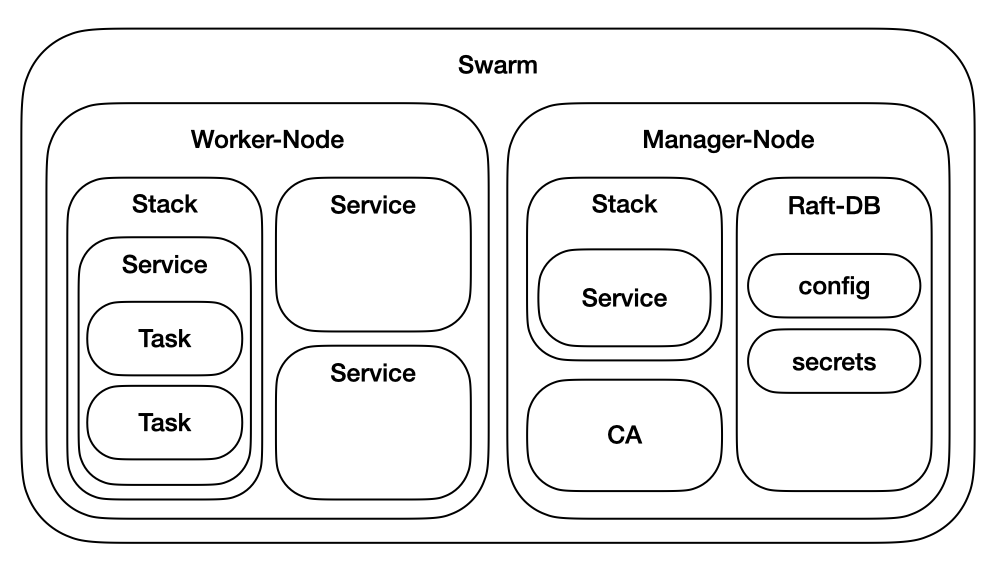
\includegraphics[width=0.7\textwidth]{figures/SwarmArchitecture.png}
    \caption{\"Ubersicht des architektonischen Aufbaus eines Docker Swarms}
    \label{fig:docker-swarm-architecture}
\end{figure}

\section{Services und Tasks}

Eine weitere logische Einheit in einem Docker Swarm nach den Nodes sind die Services. 
Diese sind oft einzelne Microservices im Kontext einer gr\"o{\ss}eren Anwendung, z.B.\ das Front- und Backend einer Anwendung oder auch eine Datenbank. 
Wie im Codebeispiel~\ref{lst:Compose} gezeigt, wird ein Service \"uber einen Namen (``frontend'') definiert und das zu verwendende Image angegeben. 
Alle weiteren Angaben sind optional, dazu z\"ahlt unter anderem
\begin{itemize}
    \item das Netzwerk, um mehrere Services untereinander erreichbar zu machen,
    \item Unter- und Obergrenzen bez\"uglich der Hardware-Ressourcen und 
    \item der gew\"unschte Zustand des Deployments, wie die Anzahl an Replikas und unter welchen Bedingungen ein Service neugestartet werden soll.
\end{itemize}

Wenn ein so definierter Service in einem Swarm ausgeführt wird, werden diese Angaben in die Raft-Datenbank der Manager-Nodes \"ubernommen, damit diese von dem Moment an den sogenannten Desired State umsetzen k\"onnen.
Das bedeutet, dass der zust\"andige Manager f\"ur jede geforderte Replika einen Task startet, der einen Container nach den genannten Vorgaben hochf\"ahrt. 
Ein Task ist somit die kleinste Verwaltungsstruktur im Docker Swarm, die genau einen Container enth\"alt und neu gestartet wird, wenn der Container den Anforderungen in der Service-Definition nicht mehr gen\"ugt, also z.B.\ wenn der Container abst\"urzt.
Die Tasks werden auf die verf\"ugbaren Worker-Nodes je nach deren Auslastung verteilt.\cite{Docker_Engine_Services}

\lstinputlisting[language=bash,caption={Compose-File zur Auslieferung eines Frontend-Services als Stack},captionpos=b,label=lst:Compose]{listings/docker-compose.yaml}

\section{Deklarativer Ansatz}

Um den gew\"unschten Zustand der Services innerhalb eines Swarms festzulegen, verwendet die Docker Engine einen deklarativen Ansatz. 
Das bedeutet, dass ein Service innerhalb einer Compose-Datei, in der Regel als yaml, definiert wird. 
In dieser Datei stehen alle Informationen, die der Manager-Node ben\"otigt, um den Service zu starten und bei Bedarf zu reparieren. 
Zu beachten ist dabei, dass die Compose-Datei im Legacy-Format Compose file version 3 sein muss, wenn der Service als Stack ausgeliefert werden soll. 
Ein Stack dient dabei der einfacheren Auslieferung von mehreren Services als Gesamtpaket und ist vergleichbar mit Docker Compose f\"ur die lokale Entwicklung.\cite{Docker_Engine_deploy}